\documentclass[a4paper,12pt]{article}

\usepackage[
    left=2cm,
    right=2cm,
    top=3cm,
    bottom=3cm
]{geometry}

\usepackage[utf8]{inputenc}
\usepackage[czech]{babel}
\usepackage[T1]{fontenc}
\usepackage{graphicx}
\usepackage{array}
\usepackage{booktabs}
\usepackage{tabularx}
\usepackage{makecell}
\usepackage{float}
\usepackage{newunicodechar}
\usepackage{url}
\usepackage{siunitx}
\usepackage{listings}
\usepackage{xcolor}
\usepackage{diagbox}
\usepackage{hyperref}
\usepackage{tikz}

\usepackage{fancyhdr}
\pagestyle{fancy}

\fancyhf{}
\fancyhead[L]{Fraunhoferův ohyb světla na štěrbině a~mřížce}
\fancyhead[R]{Pavel Pernička}
\fancyfoot[C]{\thepage}

\fancypagestyle{firstpage}{
    \fancyhf{}
    \renewcommand{\headrulewidth}{0pt}
    \renewcommand{\footrulewidth}{0pt}
    \fancyfoot[C]{\thepage}
}
\definecolor{myblue}{RGB}{111,0,248}
\newcommand{\colorcircle}[1]{%
  \tikz[baseline=-0.6ex]\draw[fill=#1,draw=none] (0,0) circle (1.5ex);%
}
\newcommand{\unitC}{\,^\circ\mathrm{C}}
\newcommand{\unitV}{\,\mathrm{V}}
\newcommand{\unitA}{\,\mathrm{A}}
\newcommand{\units}{\,\mathrm{s}}
\newcommand{\unitmin}{\,\mathrm{min}}

\newcommand{\centered}[1]{\begin{tabular}{l} #1 \end{tabular}}

\addto\captionsczech{\renewcommand{\refname}{Seznam použité literatury}}
\addto\captionsczech{\renewcommand{\figurename}{\textbf{Obrázek}}}
\addto\captionsczech{\renewcommand{\tablename}{\textbf{Tabulka}}}
\renewcommand{\lstlistingname}{\textbf{Kód}}

\lstset{
    language=Python,
    basicstyle=\ttfamily\footnotesize,
    keywordstyle=\color{blue},
    commentstyle=\color{gray},
    stringstyle=\color{red},
    numbers=left,
    numberstyle=\tiny\color{gray},
    stepnumber=1,
    breaklines=true,
    frame=single
}

\begin{document}
\thispagestyle{firstpage}

\vspace*{\fill}
\begin{center}
\renewcommand{\arraystretch}{1.75}

\begin{tabularx}{\textwidth}{|X|X|X|}
    \hline
    \multicolumn{1}{|c|}{\rule{0pt}{2.25cm} 
\includegraphics[height=2cm]{img/ctu_logo.png}}
    & \multicolumn{2}{c|}{\makecell{\textbf{KATEDRA FYZIKY}}} \\
    \hline
    \multicolumn{3}{|c|}{\Large \textbf{\centered{LABORATORNÍ CVIČENÍ Z FYZIKY}}} \\
    \hline
    \multicolumn{2}{|X}{\small{Jméno} \newline \textbf{Pavel Pernička}}
    & \multicolumn{1}{|X|}{\small{Datum měření} \newline \textbf{11.11.2025}} \\
    \hline
    {\small{Semestr} \newline \textbf{Zimní 2025}}
    & {\small{Ročník} \newline \textbf{2.}}
    & {\small{Datum odevzdání} \newline \textbf{23.12.2025}} \\
    \hline
    {\small{Stud. skupina} \newline \textbf{6}}
    & {\small{Lab. skupina} \newline \textbf{1061}}
    & {\small{Klasifikace} \newline} \\
    \hline
    \multicolumn{3}{|c|}{\rule{0pt}{1cm}} \\
    \hline
    \multicolumn{1}{|X|}{\small{Číslo úlohy \newline \textbf{7}}}
    & \multicolumn{2}{|p{9cm}|}{\small{Název úlohy \newline \textbf{Fraunhoferův ohyb světla na štěrbině a~mřížce}}} \\
    \hline
\end{tabularx}

\end{center}
\vspace*{\fill}

\newpage
\section{Úkol měření}
\begin{itemize}
\item Pro dvě šířky štěrbiny a dvě vlnové délky ověřte platnost vzorce pro Fraunhoferův ohyb na štěrbině.
\item Určete mřížkovou konstantu ohybové optické mřížky, měření proveďte pro dvě vlnové délky.
\item S využitím optické mřížky zjistěte vlnovou délku světla laserového ukazovátka.
\end{itemize}

\section{Seznam použitých nástrojů}
\begin{itemize}
    \item Optická lavice s měřítkem vzdálenosti optických prvků
        \begin{itemize}
            \item Velikost nejmenšího dílku : $1\ \unit{mm}$
        \end{itemize}
    \item Optická mřížka
    \item Štěrbina s nastavitelnou šířkou
        \begin{itemize}
            \item Velikost nejmenšího dílku : $1\ \unit{\mu m}$
        \end{itemize}
    \item Stínítko s měřítkem vzdálenosti
        \begin{itemize}
            \item Velikost nejmenšího dílku : $1\ \unit{mm}$
        \end{itemize}
    \item Lasery
        \begin{itemize}
            \item Červený HeNe ($\lambda_{č} = 650\ \unit{nm}$)
            \item Zelený LED ($\lambda_z = 532\ \unit{nm}$)
            \item Modrý ($\lambda_m$ máme za úkol určit)
        \end{itemize}
\end{itemize}

\newpage
\section{Ověření vzorce pro Fraunhoferův ohyb na štěrbině}

\subsection{Postup}
\begin{enumerate}
    \item Na optickou lavici umístíme červený laser a štěrbinu. Následně zapneme laser a posuneme štěrbinu do vzdálenosti $l$, při které je ohybový obrazec na stínítku ostrý.
    \item Na štěrbině zvolíme šířku $b_1$, zapneme laser a změříme vzdálenosti minim (resp. vzdálenosti okrajů maxim $a_n$) všech viditelných řádů.
    \item Totéž opakujeme pro druhou šířku $b_2$.
    \item Nahradíme červený laser za zelený a provedeme měření pro šířku $b_2$.
\end{enumerate}

\begin{figure}[H]
    \centering
    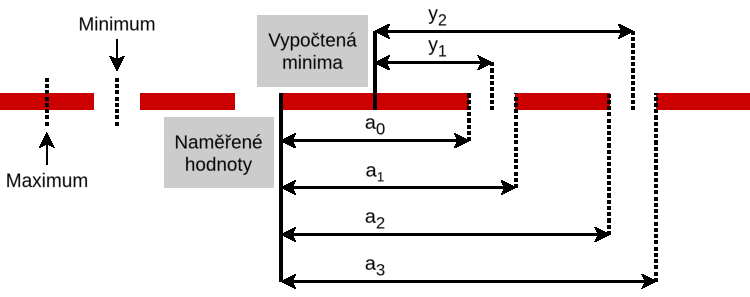
\includegraphics[width=0.95\textwidth]{img/minima.pdf}
    \caption{Schéma měřených hodnot}
    \label{fig:aparatura}
\end{figure}

\subsection{Naměřené hodnoty}

\begin{table}[H]
\centering
\renewcommand{\arraystretch}{1.5}
\begin{tabular}{|c|c|c|c|}
\hline
\multicolumn{1}{|c|}{} &
\multicolumn{2}{c|}{\textbf{Červený laser}} &
\textbf{Zelený laser} \\
\hline
$n$ &
$a_n\unit{[mm]} \; (b_1 = 0{,}35\,\text{mm})$ &
$a_n\unit{[mm]} \; (b_2 = 0{,}7\,\text{mm})$ &
$a_n\unit{[mm]} \; (b_2 = 0{,}7\,\text{mm})$ \\
\hline
0 & 18 & 6  & 6  \\
\hline
1 & 22 & 8  & 7  \\
\hline
2 & 32 & 11 & 9  \\
\hline
3 & 35 & 13 & 10 \\
\hline
4 & -- & 15 & 12 \\
\hline
5 & -- & -- & 13 \\
\hline
\end{tabular}
\label{tab:sterbina_hodnoty}
\caption{Naměřené vzdálenosti $a_n$ pro červený a zelený laser při vzdálenosti štěrbiny~$l_1=324\ \unit{mm}$ a šířky štěrbiny $b_1$ a $b_2$}
\end{table}

Z jednotlivých vzdáleností okrajů maxim vypočítáme vzdálenosti minim pomocí následujícího vztahu:
$$
y_n = \frac{a_{2n-1} + a_{2n-2}}{2} - \frac{a_0}{2}, \qquad n = 1,2,3,\dots
$$
a zobrazíme v tabulce \ref{tab:sterbina_prepocet}.

\begin{table}[H]
\centering
\renewcommand{\arraystretch}{1.5}
\begin{tabular}{|c|c|c|c|}
\hline
\multicolumn{1}{|c|}{} &
\multicolumn{2}{c|}{\textbf{Červený laser}} &
\textbf{Zelený laser} \\
\hline
$n$ &
$y_n\unit{[mm]} \; (b_1 = 0{,}35\,\text{mm})$ &
$y_n\unit{[mm]} \; (b_2 = 0{,}7\,\text{mm})$ &
$y_n\unit{[mm]} \; (b_2 = 0{,}7\,\text{mm})$ \\
\hline
1 & 11   & 4   & 3{,}5 \\
\hline
2 & 24{,}5 & 9   & 6{,}5 \\
\hline
3 & --   & --  & 9{,}5 \\
\hline
\end{tabular}
\label{tab:sterbina_prepocet}
\caption{Vypočítané vzdálenosti minim $y_n$ pro červený a zelený laser}
\end{table}


\subsection{Ověření vzorce}
Máme za úkol ověřit následující vztah:
$$
b \sin{\varphi_m} = m\lambda \qquad m=0,1,2,\dots
$$

$$
\sin \varphi_m = \frac{y_n}{\sqrt{y_n^2 + l^2}}
$$
kde $b$ je šířka štěrbiny, $\lambda$ je vlnová délka světla, $m=n$ je řád minima, $y_n$ je vzdálenost minima od středu interferenčního obrazce a $l$ je vzdálenost štěrbiny od stínítka.

Abychom mohli tento vztah ověřit, budeme se snažit podle něj vypočítat námi známou šířku štěrbiny $b$ a tu srovnáme s reálnou hodnotou. K tomuto účelu si upravíme vzorec na:

$$
b = n\lambda \cdot \frac{\sqrt{y_n^2 + l^2}}{y_n}
$$

Přístrojovou nejistota měření $u_b$ bude u všech veličin stejná, protože jak měřítko na stínítku, tak to na optické lavici, mají stejnou velikost nejmenšího dílku $\Delta = 1\ \unit{mm}$. Tedy:

$$
u_b = \frac{\Delta}{\sqrt{3}} = \frac{1}{\sqrt{3}}\ \unit{mm}
$$

Nejistotu $u_c$ získáme pomocí parciálních derivací:

$$
u_c = \sqrt{\left (\frac{\partial b}{\partial y_n}\right)^2 u_b^2(y_n) + \left (\frac{\partial b}{\partial l}\right)^2 u_b^2(l)} = \sqrt{\left(\frac{m\lambda l^2}{y_n^2 \sqrt{y_n^2 + l^2}} \right)^2 u_b^2(y_n) + \left(\frac{m\lambda l}{y_n \sqrt{y_n^2 + l^2}} \right)^2 u_b^2(y_n)}
$$

\begin{table}[H]
\centering
\renewcommand{\arraystretch}{1.5}
\begin{tabular}{|c|c|c|c|}
\hline
\multicolumn{1}{|c|}{} &
\multicolumn{2}{c|}{\textbf{Červený laser}} &
\textbf{Zelený laser} \\
\hline
$n$ &
$b_1\unit{[mm]}$ &
$b_2\unit{[mm]}$ &
$b_2\unit{[mm]}$ \\
\hline
1 &
$0{,}019 \pm 0{,}001$ &
$0{,}0527 \pm 0{,}0076$ &
$0{,}0493 \pm 0{,}0081$ \\
\hline
2 &
$0{,}01724 \pm 0{,}00041$ &
$0{,}047 \pm 0{,}003$ &
$0{,}0530 \pm 0{,}0047$ \\
\hline
3 &
-- &
-- &
$0{,}0545 \pm 0{,}0033$ \\
\hline
\end{tabular}
\caption{Vypočítané hodnoty šířky štěrbiny $b$ z naměřených hodnot}
\label{tab:sterbina_b_s_nejistotou}
\end{table}


\section{Určení mřížkové konstanty a vlnové délky laseru}
\subsection{Postup}
\begin{itemize}
    \item Na optické lavici vyměníme přípravek se štěrbinou za přípravek s optickou mřížkou. Následně zapneme laser a posuneme mřížku do vzdálenosti $l$, při které je ohybový obrazec na stínítku ostrý.
    \item Měříme vzdálenosti maxim $y_n$ pro červený, zelený i modrý laser.
\end{itemize}

\subsection{Naměřené hodnoty}

\begin{table}[H]
\centering
\renewcommand{\arraystretch}{1.5}
\begin{tabular}{|c|c|c|c|}
\hline
$n$ &
\textbf{Červený laser} $y_n\unit{[mm]}$&
\textbf{Zelený laser} $y_n\unit{[mm]}$&
\textbf{Modrý laser} $y_n\unit{[mm]}$ \\
\hline
1 & 16 & 14 & 10 \\
\hline
2 & 33 & 28 & 21 \\
\hline
3 & 50 & 42 & 32 \\
\hline
4 & 67 & 51 & 43 \\
\hline
5 & 84 & 70 & 54 \\
\hline
\end{tabular}
\caption{Vzdálenosti maxim interferenčního obrazce pro různé lasery při vzdálenosti mřížky $l_m=495\ \unit{mm}$}
\end{table}

\subsection{Mřížková konstanta}
Mřížkovou konstantu $d$ určíme pomocí podobných vztahů jako v případě ohybu na štěrbině, jen s rozdílem, že budeme používat vzdálenosti maxim místo minim. Výpočet nejistot tím pádem zůstane totožný.

$$
d = n\lambda \cdot \frac{\sqrt{y_n^2 + l^2}}{y_n}
$$

Pomocí tohoto vztahu vypočítáme tabulku \ref{tab:mrizkova_konstanta}.

\begin{table}[H]
\centering
\renewcommand{\arraystretch}{1.5}
\begin{tabular}{|c|c|c|}
\hline
$n$ &
\textbf{Červený laser} $d\ \unit{[mm]}$&
\textbf{Zelený laser} $d\ \unit{[mm]}$\\
\hline
1 & $20{,}12 \pm 0{,}73$ & $18{,}82 \pm 0{,}78$ \\
\hline
2 & $19{,}54 \pm 0{,}34$ & $18{,}84 \pm 0{,}39$ \\
\hline
3 & $19{,}40 \pm 0{,}22$ & $18{,}88 \pm 0{,}26$ \\
\hline
4 & $19{,}38 \pm 0{,}17$ & $20{,}76 \pm 0{,}23$ \\
\hline
5 & $19{,}43 \pm 0{,}13$ & $19{,}00 \pm 0{,}16$ \\
\hline
\end{tabular}
\caption{Vypočítané mřížkové konstanty $d$ pro červený a zelený laser}
\label{tab:mrizkova_konstanta}
\end{table}

Z těchto hodnot pomocí váženého průměru získáme reprezentativní hodnotu:

$$
d=(19,40\pm 0,07)\ \unit{\mu m}.
$$

\subsection{Vlnová délka modrého laseru}
Jelikož jsme si v předchozím kroku vypočítali mřížkovou konstantu, můžeme použít vztah níže pro výpočet neznámé vlnové délky modrého laseru:

$$
\lambda_m = \frac{y_nd}{n\sqrt{y_n^2+l_m^2}}
$$

Kde $n$ je řád maxima a $l_m = 495\ \unit{mm}$ je vzdálenost mřížky od stínítka. Nejistotu $u_c$ vypočítáme tímto způsobem:

$$
u_c(\lambda_m) =
\sqrt{
\left(\frac{\partial \lambda_m}{\partial d}\,u_b(d)\right)^2
+
\left(\frac{\partial \lambda_m}{\partial y_n}\,u_b(y_n)\right)^2
+
\left(\frac{\partial \lambda_m}{\partial l}\,u_b(l)\right)^2
}
$$

$$
u_c(\lambda_m) =
\sqrt{
\left(
\frac{y_n}{n\sqrt{y_n^2 + l^2}}u_b(d)
\right)^2
+
\left(
\frac{d l^2 \sqrt{y_n^2 + l^2}}{l^4 n + 2 l^2 n y_n^2 + n y_n^4}u_b(y)
\right)^2
+
\left(
\frac{d l y_n}{(n y_n^2 + l^2 n)\sqrt{y_n^2 + l^2}}\,u_b(l)
\right)^2
}.
$$

Dosazením pro jednotlivé $n$ dostáváme tabulku \ref{tab:lambda_modry}:

\begin{table}[H]
\centering
\renewcommand{\arraystretch}{1.5}
\begin{tabular}{|c|c|c|}
\hline
$n$ & $y_n\ \unit{[mm]}$ & $\lambda_m\ \unit{[nm]}$ \\
\hline
1 & 10 & $391{,}80 \pm 22{,}73$ \\
\hline
2 & 21 & $411{,}11 \pm 11{,}37$ \\
\hline
3 & 32 & $417{,}17 \pm 7{,}72$ \\
\hline
4 & 43 & $419{,}72 \pm 5{,}79$ \\
\hline
5 & 54 & $420{,}77 \pm 4{,}71$ \\
\hline
\end{tabular}
\caption{Vypočtené hodnoty vlnové délky modrého laseru z jednotlivých poloh interferenčních maxim}
\label{tab:lambda_modry}
\end{table}

Pro výpočet reprezentativní hodnoty opět použijeme vážený průměr, abychom kompenzovali vyšší nejistoty u nižších řádů $n$ a získáme:
$$
\lambda_m = (418{,}57 \pm 3{,}14)\,\unit{nm}. 
$$

\section{Závěr}
Vzorec pro Fraunhoferův ohyb na štěrbině se nám bohužel nepodařilo ověřit, neboť vypočtené hodnoty šířky štěrbiny vycházejí řádově jinak, než byla realita. Tento výstup je způsoben tím, že při měření minim na ohybovém obrazci se nám nepodařilo nastavit optickou aparaturu tak, abychom měli dostatečně široký a zároveň ostrý obraz na stínítku, takže měření bylo zatíženo výrazně větší chybou, než je vyčíslena. Další pravděpodobný důvod je to, že jsme zvolili příliš široké štěrbiny. 

Část s mřížkovou konstantou byla úspěšnější, zde se nám podařilo získat snadno měřitelný obrazec na stínítku a měření maxim bylo výrazně snazší. Z naměřených hodnot jsme získali konstantu:

$$
d=(19,40\pm 0,07)\ \unit{\mu m}.
$$

Pomocí ní jsme mohli určit vlnovou délku modrého laseru, která nám vyšla následovně:

$$
\lambda_m = (418{,}57 \pm 3{,}14)\,\unit{nm},\ \colorcircle{myblue}
$$
což spadá do fialovo-modré části spektra, a tedy to potvrzuje i správné určení mřížkové konstanty. 

\newpage

\section{Přílohy}
\begin{itemize}
    \item Foto záznamového papíru s hodnotami
\end{itemize}

\begin{thebibliography}{}

    \bibitem{zadani}
    Milan Červenka. \textit{Fraunhoferův ohyb světla na štěrbině a~mřížce}. Laboratorní úloha, 2015. Dostupné online: \url{https://planck.fel.cvut.cz/praktikum/downloads/navody/ohsvetla.pdf}.

    \bibitem{skripta}
    Michal Bednařík. \textit{Studijní texty k předmětu Fyzika 2}.
    
    \bibitem{zpracdat}
    Milan Červenka. \textit{Zpracování fyzikálních měření}. Studijní text pro fyzikální praktikum, 2020. Dostupné online: \url{https://planck.fel.cvut.cz/praktikum/downloads/navody/zpracdat.pdf}.

\end{thebibliography}

\end{document}
